%----------------------------------------------------------------
%
%  File    :  chapter3.tex
%
%  Authors :  Keith Andrews, IICM, TU Graz, Austria
%             Manuel Koschuch, FH Campus Wien, Austria
% 
%  Created :  22 Feb 96
% 
%  Changed :  30 Oct 2008
%  !TEX root = ./thesis.tex
%----------------------------------------------------------------


\chapter{Entwicklung der MCKB Applikation}
\label{chap:xamarinformsdevelopment}

	Als Basis für diese Arbeit dienen zwei während des Studiums entwickelte Applikationen.
	\begin{enumerate}
		\setlength\itemsep{0em}
		\item \textbf{STM32KB}\footnote{Download via http://m4xwe11o.ddns.net/MAD-Test/App/stm32kb.apk} - Mit Android Studio, in JAVA, entwickelte Applikation im 4. Semester an der FH Campus Wien
		\item \textbf{STM32CP} - Mit Visual Studio for Mac, in C\#, entwickelte Cross-Plattform Variante im 5. Semester an der FH Campus Wien
	\end{enumerate}
	Erstere Applikation wurde im Zuge der \textbf{Mobile App Development (MAD)} Vorlesung, zur Vertiefung von Software Engineering Skils unter Android Studio in JAVA entwickelt. Diese App ermöglicht die Darstellung von Artikeln zur Programmierung eines Microcontroller $\mu$C der Firma STM, um häfige Fragen zur Konfiguration unterschiedlicher Funktionen wie zum Beispiel \textit{UART (Universal Asynchronous Receive and Transmit)}, \textit{ADC (Analogue Digital Converter)} oder \textit{CAN (Controller Area Network)} einfach erklärt nachzulesen. Die App selber stellt nur die in einer MySQL Datenbank gespeicherten Artikel dar und ermöglichte es angemeldeten Benutzern bestehende Artikel zu editieren und zu speichern.

	Da die STM32KB App selber keine Daten speichert sondern nur darstellt wurde eine Infrastruktur entworfen um die für die App notwendigen Daten mobil abrufen zu können. Es wurde eine unter anderem eine MySQL Datenbank und ein Webserver auf einem Raspberry PI B+ eingerichtet. Neue Artikel konnten über eine PHP Webseite\footnote{http://m4xwe11o.ddns.net/MAD-Test/webwriter.php} in die Datenbank geschrieben werden. Die App lud die Artikel aus der MySQL Datenbank über verschiedenste PHP Dateien in eine lokale SQL-Lite Datenbank.

	Für die Entwicklung der STM32CP App (geschrieben mit Xamarin.Native) greift auch diese App auf die schon bestehende Infrastruktur an Server und Datenbank zurück um die Spezifizierten funktionalen Anforderungen zu erfüllen.

	\newpage
	Entsprechend der Anforderungen an die STM32KB App wurden folgende Funktionale Anforderungen im dazugehörigen \textit{Software Requirements Document (SRS)} festgehalten:
	\begin{itemize}
		\setlength\itemsep{0em}
		\item \textbf{Autor login} - Benutzer können sich in der App anmelden und sehen einen EDIT Button bei Artikeln
		\item \textbf{Autor registrieren} - Anwender können sich registrieren um als Autoren freigeschaltet zu werden
		\item \textbf{Artikel lesen} - Benutzer können Artikel lesen
	\end{itemize}

	In Abbildung \ref{fig:stm32kbApp} sind jene funktionale Anforderungen mit deren Layouts aus der App dargestellt. Die Menüführung erfolgt großteils über Buttons und der Zurück Funktion von Android über den Pfeil links oben oder jener entsprechenden Taste auf dem Android Gerät.

	\begin{figure}[h!]
		\centering
		\begin{subfigure}
			\centering
			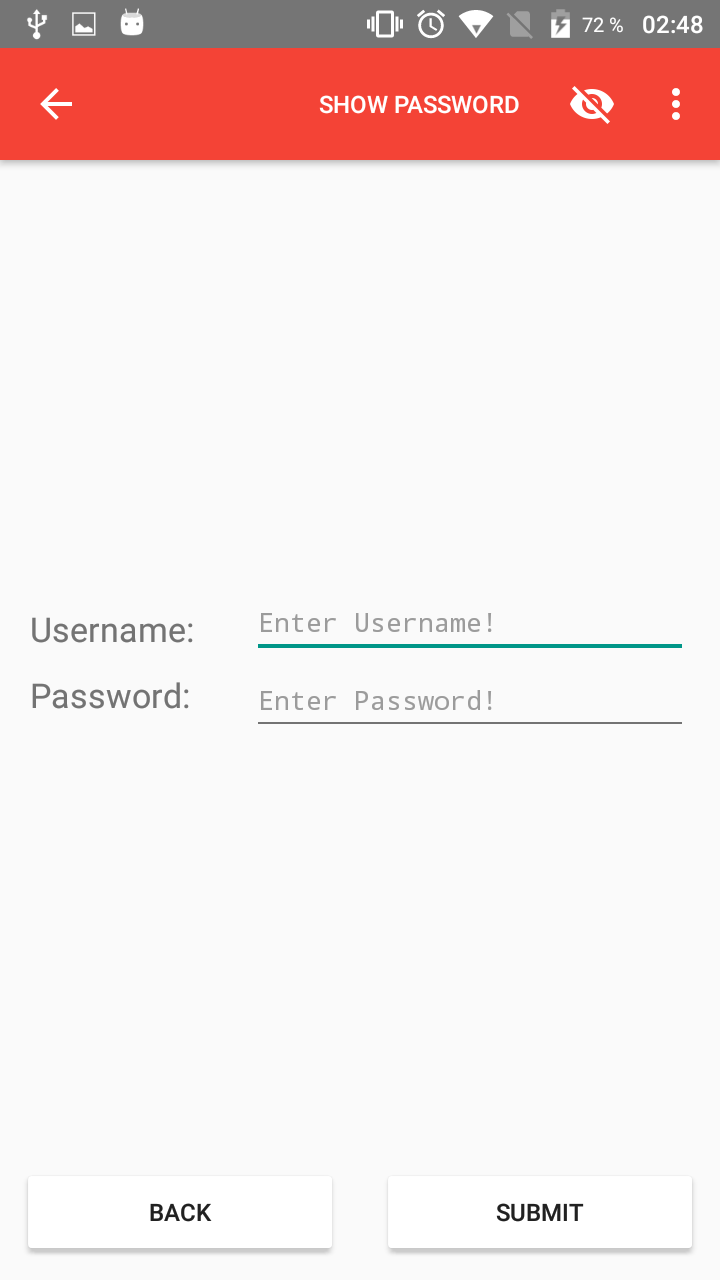
\includegraphics[width=.3\textwidth]{images/stm32kb-loginscreen.png}
		\end{subfigure}
		\begin{subfigure}
			\centering
			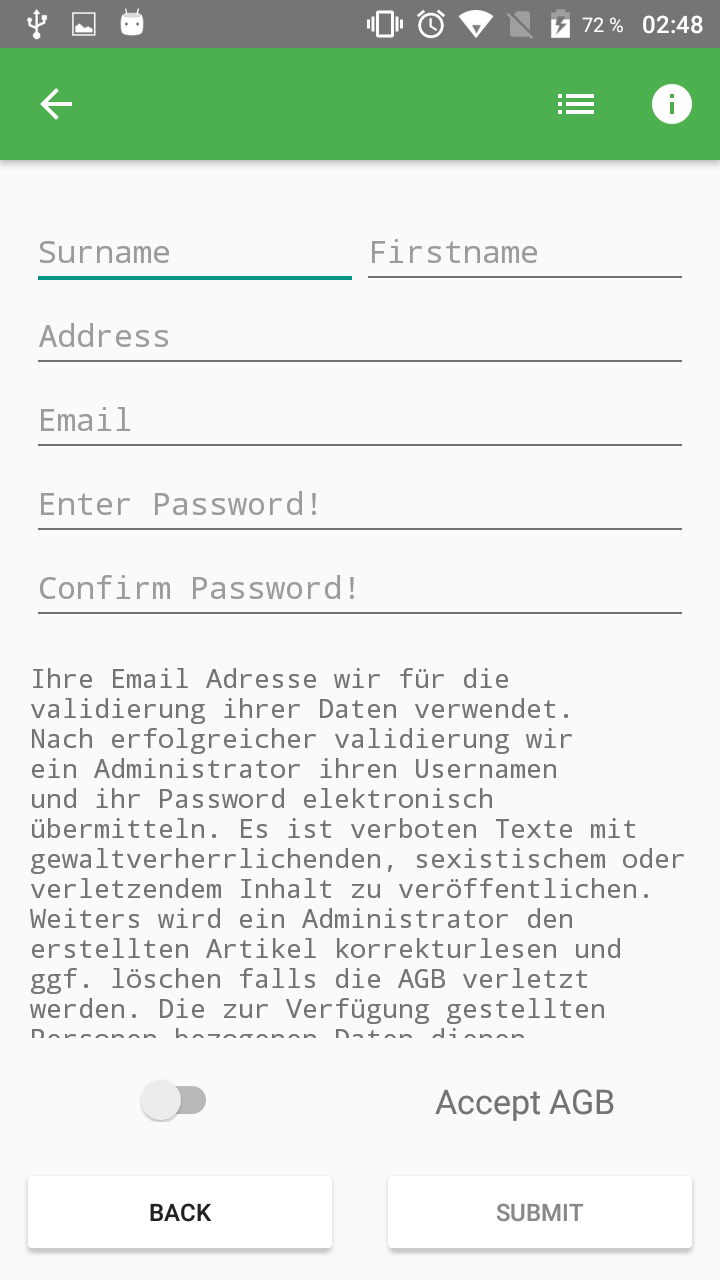
\includegraphics[width=.3\textwidth]{images/stm32kb-registerscreen.png}
		\end{subfigure}
		\begin{subfigure}
			\centering
			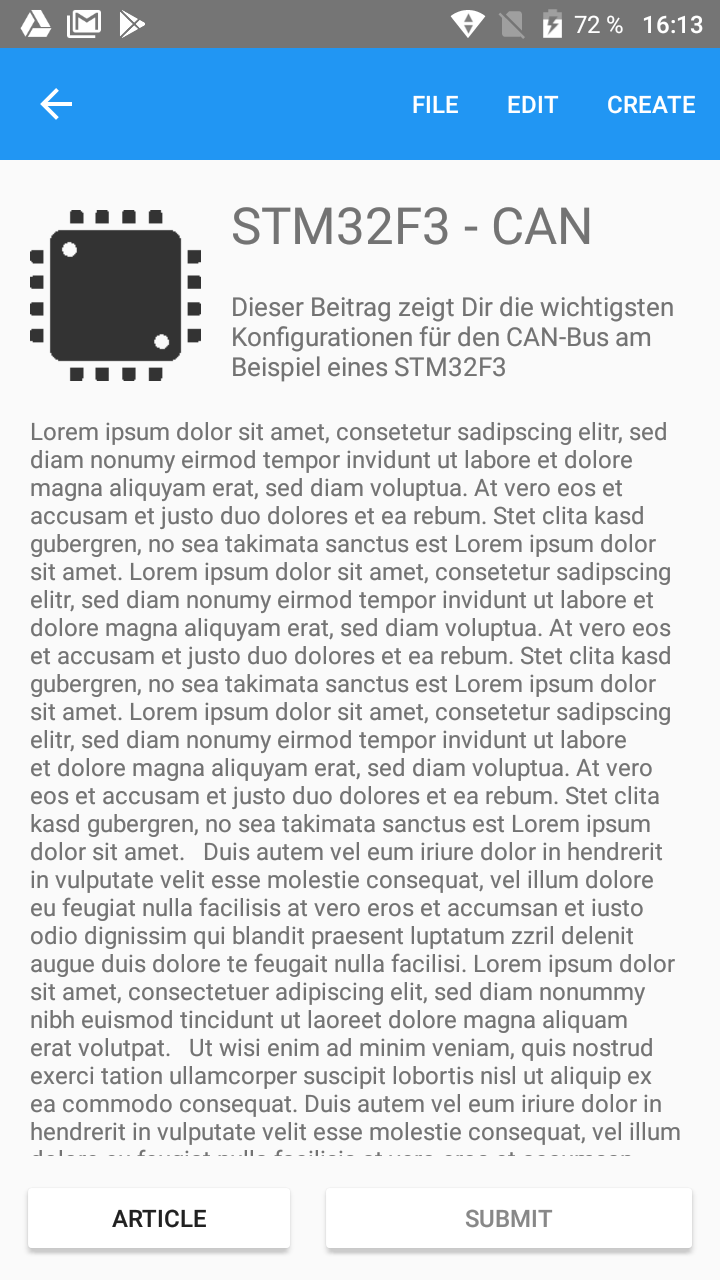
\includegraphics[width=.3\textwidth]{images/stm32kb-articlescreen.png}
		\end{subfigure}
		\caption{Design der STM32KB App - v.l.n.r. Login, Register, Lesen}
		\label{fig:stm32kbApp}
	\end{figure}

	Für die Entwicklung beider CP-Apps wurde eine andere Art der Menüführung herangezogen. Statt einer Navigation über Buttons und Pfeile sind die funktionalen Anforderungen in Form von Tabs umgesetzt worden. Ein Tabbed Layout steht sowohl unter Xamarin.Native als auch Xamarin.Forms zur Verfügung und wird von dem jeweiligen Zielbetriebssystem Renderer so gerendert das es dem Typischen Design Merkmalen entspricht.

\section{Applikations Spezifizierung}
\label{sec:mckspecs}

\subsection{Funktionale Anforderungen}
\label{sec:mckbfunkcspecs}

\subsection{Nicht Funktionale Anforderungen}
\label{sec:mckbnonfuncspecs}

\section{Unterschiede zur Xamarin.Native Version}
\label{sec:mckbspecs}














